\documentclass[5p,sort&compress]{elsarticle}

\usepackage{amssymb}    % Mathematical symbols
\usepackage{amsmath}    % More options for mathematics
\usepackage{subfigure}  % More options for figures
\usepackage{epstopdf}   % Convert eps to pdf
\usepackage[separate-uncertainty=true]{siunitx}   % Proper formatting of units in math mode
\usepackage{color}      % Supports text color if needed
\usepackage{soul}       % https://ctan.org/pkg/soul
\usepackage{lmodern}    % Loading fonts
\usepackage{hyperref}   % To insert clickable references/urls
\usepackage{listings}   % To input code in the text
\usepackage{amsmath}
\usepackage{amsmath}
\usepackage{amssymb}
\usepackage{graphicx}
\usepackage{epstopdf}
\usepackage{booktabs}
\setlength{\parskip}{2em}
\newcommand{\stirlingii}{\genfrac{\{}{\}}{0pt}{}}

% Choose the style of the reference list (do not change)
\bibliographystyle{elsarticle-num}

\journal{ifding/learning-notes}

% Begin the document

\begin{document}

\begin{frontmatter}
    \title{Ch 9: Mixture Models and EM}
    \author{ifding}
    
    \begin{abstract}
        K-means Clustering, Mixtures of Gaussians
    \end{abstract}


\end{frontmatter}

%% How to make a heading and divide the documents into different sections

If we define a joint distribution over observed and latent variables, the corresponding distribution of the observed variables alone is obtained by marginalization.


\section{K-means Clustering}

Suppose we have a data set $\{\mathbf{x}_1, \ldots, \mathbf{x}_N\}$ consisting of N observations of a random D-dimensional Euclidean variable $\mathbf{x}$. Our goal is to partition the data set into some number K of clusters.  A set of $D-$dimensional vectors $\boldsymbol{\mu}_k$, where $k=1, \ldots, K$, in which $\boldsymbol{\mu}_k$ is a prototype associated with the $k^{th}$ cluster.

For each data point $\mathbf{x}_n$, we introduce a corresponding set of binary indicator variables $r_{n k} \in \{0, 1\}$, where $k=1, \ldots, K$ describing which of the K clusters the data point $\mathbf{x}_n$ is assigned to, so that if data point $\mathbf{x}_n$ is assigned to cluster k then $r_{nk} = 1$, and $r_{nj} = 0$ for $j \neq k$.
\begin{equation}
J=\sum_{n=1}^{N} \sum_{k=1}^{K} r_{n k}\left\|\mathbf{x}_{n}-\boldsymbol{\mu}_{k}\right\|^{2}
\end{equation}
which represents the sum of the squares of the distances of each data point to its assigned vector $\boldsymbol{\mu}_k$. Our goal is to find values for the $\{r_{nk}\}$ and the $\{\boldsymbol{\mu}_k\}$ so as to minimize $J$.

We can do this through an iterative procedure in which each iteration involves two successive steps. First we choose some initial values for the $\boldsymbol{\mu}_k$. Then in the first phase we minimize $J$ with respect to the $r_{nk}$, keeping the $\boldsymbol{\mu}_k$ fixed. In the second phase we minimize $J$ with respect to the $\boldsymbol{\mu}_k$, keeping $r_{nk}$ fixed. This two-stage optimization is then repeated until convergence. These two stages of updating $r_{nk}$ and updating $\boldsymbol{\mu}_k$ correspond respectively to the E (expectation) and M (maximization) steps of the EM algorithm.

Consider first the determination of the $r_{nk}$, we simply assign the $n^{th}$ data point to the closest cluster centre.
\begin{equation}
r_{n k}=\left\{\begin{array}{ll}{1} & {\text { if } k=\arg \min _{j}\left\|\mathbf{x}_{n}-\boldsymbol{\mu}_{j}\right\|^{2}} \\ {0} & {\text { otherwise }}\end{array}\right.
\end{equation}

Now consider the optimization of the $\boldsymbol{\mu}_k$ with the $r_{nk}$ held fixed. Set its derivative with respect to $\boldsymbol{\mu}_k$ to zero giving
\begin{equation}
2 \sum_{n=1}^{N} r_{n k}\left(\mathbf{x}_{n}-\boldsymbol{\mu}_{k}\right)=0
\end{equation}
which we can easily solve for $\boldsymbol{\mu}_k$ to give
\begin{equation}
\boldsymbol{\mu}_{k}=\frac{\sum_{n} r_{n k} \mathbf{x}_{n}}{\sum_{n} r_{n k}}
\end{equation}
The denominator in this expression is equal to the number of points assigned to cluster $k$, and set $\boldsymbol{\mu}_k$ equal to the mean of all of the data points $\mathbf{x}_n$ assigned to cluster $k$.



\section{Mixtures of Gaussians}

The Gaussian mixture distribution can be written as linear superposition of Gaussians in the form
\begin{equation}
p(\mathbf{x})=\sum_{k=1}^{K} \pi_{k} \mathcal{N}\left(\mathbf{x} | \boldsymbol{\mu}_{k}, \mathbf{\Sigma}_{k}\right)
\end{equation}
Let us introduce a $K-$dimensional binary random variable $\mathbf{z}$ having a 1-of-$K$ representation, the values of $z_k$ satisfy $z_k \in \{0,1\}$ and $\sum_k z_k = 1$. There are $K$ possible states for the vector $\mathbf{z}$ according to which element is nonzero.

\begin{figure}[ht]
     \centering
     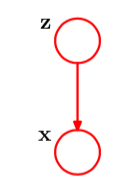
\includegraphics[width = 0.3\linewidth]{figure/figure9_4.png}
     \caption{Graphical representation of a mixture model, $p(\mathbf{x}, \mathbf{z}) = p(\mathbf{z}) p(\mathbf{x}|\mathbf{z})$.}
     \label{fig:9_4}
\end{figure}

We shall define the joint distribution $p(\mathbf{x}, \mathbf{z})$ in terms of a marginal distribution $p(\mathbf{z})$ and a conditional distribution $p(\mathbf{x}|\mathbf{z})$, corresponding to the graphical model in Figure~\ref{fig:9_4}.

The marginal distribution over $\mathbf{z}$ is specified in terms of the mixing coefficients $\pi_k$, such that
\begin{equation}
p\left(z_{k}=1\right)=\pi_{k}
\end{equation}
where the parameters $\{\pi_k\}$ must satisfy
\begin{equation}
0 \leqslant \pi_{k} \leqslant 1
\end{equation}
together with 
\begin{equation}
\sum_{k=1}^{K} \pi_{k}=1
\end{equation}
in order to be valid probabilities. Because $\mathbf{z}$ uses a 1-of-$K$ representation, we can write the distribution in the form
\begin{equation}
p(\mathbf{z})=\prod_{k=1}^{K} \pi_{k}^{z_{k}}
\end{equation}
The conditional distribution of $\mathbf{x}$ given a particular value for $\mathbf{z}$ is a Gaussian
\begin{equation}
p\left(\mathbf{x} | z_{k}=1\right)=\mathcal{N}\left(\mathbf{x} | \boldsymbol{\mu}_{k}, \mathbf{\Sigma}_{k}\right)
\end{equation}
which can also be written in the form
\begin{equation}
p(\mathbf{x} | \mathbf{z})=\prod_{k=1}^{K} \mathcal{N}\left(\mathbf{x} | \boldsymbol{\mu}_{k}, \mathbf{\Sigma}_{k}\right)^{z_{k}}
\end{equation}
\begin{equation}
p(\mathbf{x})=\sum_{\mathbf{z}} p(\mathbf{x} | \mathbf{z}) p(\mathbf{z})=\sum_{\mathbf{z}} \prod_{k=1}^{K}\left(\pi_{k} \mathcal{N}\left(\mathbf{x} | \boldsymbol{\mu}_{k}, \mathbf{\Sigma}_{k}\right)\right)^{z_{k}}
\end{equation}
Exploiting the 1-of-$K$ representation for $\mathbf{z}$, we can re-write the r.h.s. as
\begin{equation}
\sum_{j=1}^{K} \prod_{k=1}^{K}\left(\pi_{k} \mathcal{N}\left(\mathbf{x} | \boldsymbol{\mu}_{k}, \mathbf{\Sigma}_{k}\right)\right)^{I_{k j}}=\sum_{j=1}^{K} \pi_{j} \mathcal{N}\left(\mathbf{x} | \boldsymbol{\mu}_{j}, \mathbf{\Sigma}_{j}\right)
\end{equation}
where $\mathbf{I}_{kj} = 1$ if $k = j$ and 0 otherwise. The marginal distribution of $\mathbf{x}$ is a Gaussian mixture.

The conditional probability of $\mathbf{z}$ given $\mathbf{x}$, we shall use $\gamma(z_k)$ to denote $p(z_k = 1 | \mathbf{x})$,
\begin{equation}
\begin{aligned} \gamma\left(z_{k}\right) \equiv p\left(z_{k}=1 | \mathbf{x}\right)=& \frac{p\left(z_{k}=1\right) p\left(\mathbf{x} | z_{k}=1\right)}{K} \\ & \sum_{j=1}^{K} p\left(z_{j}=1\right) p\left(\mathbf{x} | z_{j}=1\right) \\=& \frac{\pi_{k} \mathcal{N}\left(\mathbf{x} | \boldsymbol{\mu}_{k}, \mathbf{\Sigma}_{k}\right)}{\sum_{j=1}^{K} \pi_{j} \mathcal{N}\left(\mathbf{x} | \boldsymbol{\mu}_{j}, \mathbf{\Sigma}_{j}\right)} \end{aligned}
\end{equation}
We shall view $\pi_k$ as the prior probability of $z_k = 1$, and the quantity $\gamma (z_k)$ as the corresponding posterior probability once we have observed $\mathbf{x}$. $\gamma (z_k)$ can also be viewed as the \textit{responsibility} that component $k$ takes for `explaining' the observation $\mathbf{x}$.


\subsection{Maximum likelihood}

Suppose we have a data set of observations $\{\mathbf{x}_1, \ldots, \mathbf{x}_N\}$, and we wish to model this data using a mixture of Gaussians. We can represent this data set as an $N \times D$ matrix $\mathbf{X}$ in which the $n^{th}$ rows is given by $\mathbf{x}_n^{\mathrm{T}}$. The corresponding latent variables will be denoted by an $N \times K$ matrix $\mathbf{Z}$ with rows $\mathbf{z}_n^{\mathrm{T}}$. The log of likelihood function is given by
\begin{equation}
\ln p(\mathbf{X} | \boldsymbol{\pi}, \boldsymbol{\mu}, \mathbf{\Sigma})=\sum_{n=1}^{N} \ln \left\{\sum_{k=1}^{K} \pi_{k} \mathcal{N}\left(\mathbf{x}_{n} | \boldsymbol{\mu}_{k}, \mathbf{\Sigma}_{k}\right)\right\}
\end{equation}

The presence of \textbf{singularities}, for simplicity, consider a Gaussian mixture whose components have covariance matrices given by $\sum_k = \sigma^2 \mathbf{I}$, which $\mathbf{I}$ is the unit matrix. Suppose that one of the components of the mixture model, the $j^{th}$ component, has its mean $\boldsymbol{\mu}_j$ exactly equal to one of the data points so that $\boldsymbol{\mu}_j = \mathbf{x}_n$ for some value of $n$.
\begin{equation}
\mathcal{N}\left(\mathbf{x}_{n} | \mathbf{x}_{n}, \sigma_{j}^{2} \mathbf{I}\right)=\frac{1}{(2 \pi)^{1 / 2}} \frac{1}{\sigma_{j}}
\end{equation}
If we consider the limit $\text { limit } \sigma_{j} \rightarrow 0$, the log likelihood function will go to infinity. Thus the maximization of the log likelihood function is not a well posed problem because such singularities will always be present and will occur whenever one of the Gaussian components `collapses' onto a specific data point.


\subsection{EM for Gaussian mixtures}

Let us begin by writing down the conditions that must be satisfied at a maximum of the likelihood function. Setting the derivatives of $\ln{p(\mathbf{X}|\boldsymbol{\pi}, \boldsymbol{\mu}, \boldsymbol{\Sigma})}$ with respect to the mean $\boldsymbol{\mu}_k$ to zero,
\begin{equation}
0=-\sum_{n=1}^{N} \underbrace{\frac{\pi_{k} \mathcal{N}\left(\mathbf{x}_{n} | \boldsymbol{\mu}_{k}, \mathbf{\Sigma}_{k}\right)}{\sum_{j} \pi_{j} \mathcal{N}\left(\mathbf{x}_{n} | \boldsymbol{\mu}_{j}, \mathbf{\Sigma}_{j}\right)}}_{\gamma\left(z_{n k}\right)} \boldsymbol{\Sigma}_{k}^{-1}\left(\mathbf{x}_{n}-\boldsymbol{\mu}_{k}\right)
\end{equation}
Multiplying by $\Sigma_k^{-1}$ and rearranging we obtain
\begin{equation}
\mu_{k}=\frac{1}{N_{k}} \sum_{n=1}^{N} \gamma\left(z_{n k}\right) \mathbf{x}_{n}
\end{equation}
where we have defined
\begin{equation}
N_{k}=\sum_{n=1}^{N} \gamma\left(z_{n k}\right)
\end{equation}
We can interpret $N_k$ as the effective number of points assigned to cluster k. The mean $\boldsymbol{\mu}_k$ for the $k^{th}$ Gaussian component is obtained by taking a weighted mean of all of the points in the data set, in which the weighting factor is given by the posterior probability $\gamma(z_{nk})$ that component $k$ was responsible for generating $\mathbf{x}_n$.

If we set the derivative of $\ln{p(\mathbf{X}|\boldsymbol{\pi}, \boldsymbol{\mu}, \boldsymbol{\Sigma})}$ with respect to $\boldsymbol{\Sigma}_k$ to zero,
\begin{equation}
\mathbf{\Sigma}_{k}=\frac{1}{N_{k}} \sum_{n=1}^{N} \gamma\left(z_{n k}\right)\left(\mathbf{x}_{n}-\boldsymbol{\mu}_{k}\right)\left(\mathbf{x}_{n}-\boldsymbol{\mu}_{k}\right)^{\mathrm{T}}
\end{equation}

Finally, we maximize $\ln{p(\mathbf{X}|\boldsymbol{\pi}, \boldsymbol{\mu}, \boldsymbol{\Sigma})}$ with respect to the mixing coefficients $\pi_k$, and take account of the constraint that the mixing coefficients sum to one. 
\begin{equation}
\pi_{k}=\frac{N_{k}}{N}
\end{equation}
so that the mixing coefficient for the $k^{th}$ component is given by the average responsibility which that component takes for explaining the data points.

\subsection{EM algorithm}

1. Initialize the means $\boldsymbol{\mu}_k$, covariances $\\boldsymbol{Sigma}_k$ and mixing coefficients $\pi_k$, and evaluate the initial value of the log likelihood.

2. \textbf{E step.} Evaluate the responsibilities using the current parameter values
\begin{equation}
\gamma\left(z_{n k}\right)=\frac{\pi_{k} \mathcal{N}\left(\mathbf{x}_{n} | \boldsymbol{\mu}_{k}, \mathbf{\Sigma}_{k}\right)}{\sum_{j=1}^{K} \pi_{j} \mathcal{N}\left(\mathbf{x}_{n} | \boldsymbol{\mu}_{j}, \mathbf{\Sigma}_{j}\right)}
\end{equation}

3. \textbf{M step}. Re-estimate the parameters using the current responsibilities
\begin{equation}
\boldsymbol{\mu}_{k}^{\mathrm{new}}=\frac{1}{N_{k}} \sum_{n=1}^{N} \gamma\left(z_{n k}\right) \mathbf{x}_{n}
\end{equation}
\begin{equation}
\boldsymbol{\Sigma}_{k}^{\text {new }}=\frac{1}{N_{k}} \sum_{n=1}^{N} \gamma\left(z_{n k}\right)\left(\mathbf{x}_{n}-\boldsymbol{\mu}_{k}^{\text {new }}\right)\left(\mathbf{x}_{n}-\boldsymbol{\mu}_{k}^{\text {new }}\right)^{\mathrm{T}}
\end{equation}
\begin{equation}
\pi_{k}^{\mathrm{new}}=\frac{N_{k}}{N}
\end{equation}
where
\begin{equation}
N_{k}=\sum_{n=1}^{N} \gamma\left(z_{n k}\right)
\end{equation}

4. Evaluate the log likelihood
\begin{equation}
\ln p(\mathbf{X} | \boldsymbol{\mu}, \mathbf{\Sigma}, \boldsymbol{\pi})=\sum_{n=1}^{N} \ln \left\{\sum_{k=1}^{K} \pi_{k} \mathcal{N}\left(\mathbf{x}_{n} | \boldsymbol{\mu}_{k}, \mathbf{\Sigma}_{k}\right)\right\}
\end{equation}
and check for convergence of either the parameters or the log likelihood. If the convergence criterion is not satisfied return to step 2.


\section{An Alternative View of EM}

The goal of the EM algorithm is to find maximum likelihood solutions for models having latent variables $\mathbf{Z}$, the log likelihood function is given by
\begin{equation}
\ln p(\mathbf{X} | \boldsymbol{\theta})=\ln \left\{\sum_{\mathbf{Z}} p(\mathbf{X}, \mathbf{Z} | \boldsymbol{\theta})\right\}
\end{equation}
Note that the discussion will apply equally well to continuous latent variables simply replacing the sum over $\mathbf{Z}$ with an integral.

Suppose that, for each observation in $\mathbf{X}$, we were told the corresponding value of the latent variable $\mathbf{Z}$, $\{\mathbf{X}, \mathbf{Z}\}$ is called as the complete data set. In practice, we are only given the incomplete data $\mathbf{X}$. The values of the latent variables in $\mathbf{Z}$ is given by the posterior distribution $p(\mathbf{Z}|\mathbf{X}, \boldsymbol{\theta})$. Because we cannot use the complete data log likelihood $p(\mathbf{X}, \mathbf{Z} | \boldsymbol{\theta})$, we consider instead its expected value under the posterior distribution of the latent variable, which corresponds to the E step. 

In the E step, we use the current parameter values $\boldsymbol{\theta}^{old}$ to find the posterior distribution $p(\mathbf{Z}|\mathbf{X}, \boldsymbol{\theta}^{old})$. We then use this posterior distribution to find the expectation of the complete data log likelihood evaluated for some general parameter value $\boldsymbol{\theta}$.
\begin{equation}
\mathcal{Q}\left(\boldsymbol{\theta}, \boldsymbol{\theta}^{\text {old }}\right)=\sum_{\mathbf{Z}} p\left(\mathbf{Z} | \mathbf{X}, \boldsymbol{\theta}^{\text {old }}\right) \ln p(\mathbf{X}, \mathbf{Z} | \boldsymbol{\theta})
\end{equation}

In the M step, we determine the revised parameter estimate $\boldsymbol{\theta}^{new}$ by maximizing this function
\begin{equation}
\boldsymbol{\theta}^{\text {new }}=\underset{\boldsymbol{\theta}}{\arg \max } \mathcal{Q}\left(\boldsymbol{\theta}, \boldsymbol{\theta}^{\text {old }}\right)
\end{equation}


\subsection{Gaussian mixtures revisited}

Suppose then that in addition to the observed data set $\mathbf{X}$, we were also given the values of the corresponding discrete variables $\mathbf{Z}$. The graphical model for the complete data is shown in Figure~\ref{fig:9_9}.

\begin{figure}[ht]
     \centering
     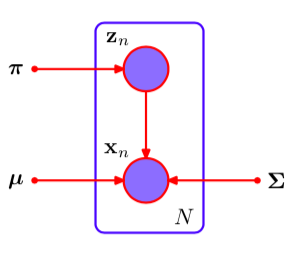
\includegraphics[width = 0.8\linewidth]{figure/figure9_9.png}
     \caption{The discrete variables $z_n$ are observed, as well as the data variables $\mathbf{x}_n$.}
     \label{fig:9_9}
\end{figure}

Now consider the problem of maximizing the likelihood for the complete data set $\{\mathbf{X}, \mathbf{Z}\}$.
\begin{equation}
p(\mathbf{X}, \mathbf{Z} | \boldsymbol{\mu}, \boldsymbol{\Sigma}, \boldsymbol{\pi})=\prod_{n=1}^{N} \prod_{k=1}^{K} \pi_{k}^{z_{n k}} \mathcal{N}\left(\mathbf{x}_{n} | \boldsymbol{\mu}_{k}, \boldsymbol{\Sigma}_{k}\right)^{z_{n k}}
\end{equation}
where $z_{nk}$ denotes the $k^{th}$ component of $\mathbf{z}_n$. Taking the logarithm
\begin{equation}
\ln p(\mathbf{X}, \mathbf{Z} | \boldsymbol{\mu}, \boldsymbol{\Sigma}, \boldsymbol{\pi})=\sum_{n=1}^{N} \sum_{k=1}^{K} z_{n k}\left\{\ln \pi_{k}+\ln \mathcal{N}\left(\mathbf{x}_{n} | \boldsymbol{\mu}_{k}, \boldsymbol{\Sigma}_{k}\right)\right\}
\end{equation}

Consider first the maximization with respect to the means and covariances. Because $\mathbf{z}_n$ is a K-dimensional vector with all elements equal to 0 except for a single element having the value 1, the complete data log likelihood function is simply a sum of K independent contributions, one for each mixture component. Thus the maximization with respect to a mean or a covariance is exactly as for a single Gaussian, except that it involves only the subset of data points that are `assigned' to that component. For the maximization with respect to the mixing coefficients, this can be enforced using a Lagrange multiplier,
\begin{equation}
\pi_{k}=\frac{1}{N} \sum_{n=1}^{N} z_{n k}
\end{equation}
the mixing coefficients are equal to the fractions of data points assigned to the corresponding components.

The complete-data log likelihood function can be maximized trivially in closed form. In practice, however, we do not have values for the latent variables. We consider the expectation, with respect to the posterior distribution of the latent variables, of the complete-data log likelihood. The posterior distribution takes the form
\begin{equation}
p(\mathbf{Z} | \mathbf{X}, \boldsymbol{\mu}, \boldsymbol{\Sigma}, \boldsymbol{\pi}) \propto \prod_{n=1}^{N} \prod_{k=1}^{K}\left[\pi_{k} \mathcal{N}\left(\mathbf{x}_{n} | \boldsymbol{\mu}_{k}, \boldsymbol{\Sigma}_{k}\right)\right]^{z_{n k}}
\end{equation}
To prove it, we only need to prove $p(\mathbf{Z}|\mathbf{X})$ can be written as the product of $p(\mathbf{z}_n | \mathbf{x}_n)$. Notice that the condition on $\boldsymbol{\mu}$, $\boldsymbol{\Sigma}$ and $\boldsymbol{\pi}$ can be omitted.
\begin{equation}
p(\mathbf{X}, \mathbf{Z})=p\left(\mathbf{x}_{1}, \mathbf{z}_{1}\right) \ldots p\left(\mathbf{x}_{N}, \mathbf{z}_{N}\right)
\end{equation}
Since there is no link from $\mathbf{z}_m$ to $\mathbf{z}_n$, from $\mathbf{x}_m$ to $\mathbf{x}_n$, and from $\mathbf{z}_m$ to $\mathbf{x}_n$ (m $\neq$ n),
\begin{equation}
p(\mathbf{Z})=p\left(\mathbf{z}_{1}\right) \ldots p\left(\mathbf{z}_{N}\right), \quad p(\mathbf{X})=p\left(\mathbf{x}_{1}\right) \ldots p\left(\mathbf{x}_{N}\right)
\end{equation}
The marginal distribution from $p(\mathbf{X}, \mathbf{Z})$
\begin{equation}
\begin{aligned}
p(\mathbf{Z})=\sum_{\mathbf{X}} p(\mathbf{X}, \mathbf{Z})=\sum_{\mathbf{x}_{1}, \ldots, \mathbf{x}_{N}} p\left(\mathbf{x}_{1}, \mathbf{z}_{1}\right) \ldots p\left(\mathbf{x}_{N}, \mathbf{z}_{N}\right) \\
=p\left(\mathbf{z}_{1}\right) \ldots p\left(\mathbf{z}_{N}\right)
\end{aligned}
\end{equation}
According to Bayes' Theorem, we have
\begin{equation}
\begin{aligned} p(\mathbf{Z} | \mathbf{X}) &=\frac{p(\mathbf{X} | \mathbf{Z}) p(\mathbf{Z})}{p(\mathbf{X})} \\ &=\frac{\left[\prod_{n=1}^{N} p\left(\mathbf{x}_{n} | \mathbf{z}_{n}\right)\right]\left[\prod_{n=1}^{N} p\left(\mathbf{z}_{n}\right)\right]}{\prod_{n=1}^{N} p\left(\mathbf{x}_{n}\right)} \\ &=\prod_{n=1}^{N} \frac{p\left(\mathbf{x}_{n} | \mathbf{z}_{n}\right) p\left(\mathbf{z}_{n}\right)}{p\left(\mathbf{x}_{n}\right)} \\ &=\prod_{n=1}^{N} p\left(\mathbf{z}_{n} | \mathbf{x}_{n}\right) \end{aligned}
\end{equation}


\subsection{Relation to K-means}

Whereas the K-means algorithm performs a \textit{hard} assignment of data points to clusters, in which each data point is associated uniquely with one cluster, the EM algorithm makes a \textit{soft} assignment based on the posterior probabilities.

Consider a Gassian mixture model in which the covariance matrices of the mixture components are given by $\epsilon\mathbf{I}$, where $\epsilon$ is a variance parameter that is shared by all of the components, and $\mathbf{I}$ is the identify matrix, so that
\begin{equation}
p\left(\mathbf{x} | \boldsymbol{\mu}_{k}, \mathbf{\Sigma}_{k}\right)=\frac{1}{(2 \pi \epsilon)^{1 / 2}} \exp \left\{-\frac{1}{2 \epsilon}\left\|\mathbf{x}-\boldsymbol{\mu}_{k}\right\|^{2}\right\}
\end{equation}
We now consider the EM algorithm for a mixture of K gaussians of this form in which we treat $\epsilon$ as a fixed constant. The posterior probabilities, or responsibilities, for a particular data point $\mathbf{x}_n$, are given by
\begin{equation}
\gamma\left(z_{n k}\right)=\frac{\pi_{k} \exp \left\{-\left\|\mathbf{x}_{n}-\boldsymbol{\mu}_{k}\right\|^{2} / 2 \epsilon\right\}}{\sum_{j} \pi_{j} \exp \left\{-\left\|\mathbf{x}_{n}-\boldsymbol{\mu}_{j}\right\|^{2} / 2 \epsilon\right\}}
\end{equation}
If we consider the limit $\epsilon \rightarrow 0$, in the denominator the term for which $\left\|\mathbf{x}_{n}-\boldsymbol{\mu}_{j}\right\|^{2}$ is smallest will go to zero most slowly, and hence the responsibilities $\gamma\left(z_{n k}\right)$ for the data point $\mathbf{x}_n$ all go to zero except for term $j$, for which the responsibility $\gamma\left(z_{n j}\right)$ will go to 1. In this limit, we obtain a hard assignment of data points to clusters, just as in the K-means algorithm. Finally, in the limit $\epsilon \rightarrow 0$ the expected complete-data likelihood becomes
\begin{equation}
\begin{aligned}
\mathbb{E}_{\mathbf{Z}}[\ln p(\mathbf{X}, \mathbf{Z} | \boldsymbol{\mu}, \boldsymbol{\Sigma}, \boldsymbol{\pi})] \rightarrow-\frac{1}{2} \sum_{n=1}^{N} \sum_{k=1}^{K} r_{n k}\left\|\mathbf{x}_{n}-\boldsymbol{\mu}_{k}\right\|^{2}+ \\
\text { const. }
\end{aligned}
\end{equation}
Thus, maximizing the expected complete-data log likelihood is equivalent to minimizing the distortion measure $J$ for the K-means algorithm.


\section{The EM Algorithm in General}

Consider a probabilistic model in which we collectively denote all of the observed variables by $\mathbf{X}$ and all of the hidden variables by $\mathbf{Z}$. The joint distribution $p(\mathbf{X}, \mathbf{Z}|\boldsymbol{\theta})$ is governed by a set of parameters denoted $\boldsymbol{\theta}$. Our goal is to maximize the likelihood function that is given by
\begin{equation}
p(\mathbf{X} | \boldsymbol{\theta})=\sum_{\mathbf{Z}} p(\mathbf{X}, \mathbf{Z} | \boldsymbol{\theta})
\end{equation}
Here we are assuming $\mathbf{Z}$ is discrete, although the discussion is identical if $\mathbf{Z}$ comprises continuous variables.

We shall suppose that direct optimization of $p(\mathbf{X}|\boldsymbol{\theta})$ is difficult, but that optimization of $p(\mathbf{X}, \mathbf{Z}|\boldsymbol{\theta})$ is easier. Next we introduce a distribution $q(\mathbf{Z})$ defined over the latent variables,
\begin{equation}\label{decomposition}
\ln p(\mathbf{X} | \boldsymbol{\theta})=\mathcal{L}(q, \boldsymbol{\theta})+\mathrm{KL}(q \| p)
\end{equation}
where we have defined
\begin{equation}
\begin{aligned} \mathcal{L}(q, \boldsymbol{\theta}) &=\sum_{\mathbf{Z}} q(\mathbf{Z}) \ln \left\{\frac{p(\mathbf{X}, \mathbf{Z} | \boldsymbol{\theta})}{q(\mathbf{Z})}\right\} \\ \mathrm{KL}(q \| p) &=-\sum_{\mathbf{Z}} q(\mathbf{Z}) \ln \left\{\frac{p(\mathbf{Z} | \mathbf{X}, \boldsymbol{\theta})}{q(\mathbf{Z})}\right\} \end{aligned}
\end{equation}
$\mathcal{L}(q, \boldsymbol{\theta})$ contains the joint distribution of $\mathbf{X}$ and $\mathbf{Z}$ while $\mathrm{KL}(q \| p)$ contains the conditional distribution of $\mathbf{}$ given $\mathbf{X}$. To verify the decomposition, we first make use of the product rule of probability to give
\begin{equation}
\ln p(\mathbf{X}, \mathbf{Z} | \boldsymbol{\theta})=\ln p(\mathbf{Z} | \mathbf{X}, \boldsymbol{\theta})+\ln p(\mathbf{X} | \boldsymbol{\theta})
\end{equation}
which we then substitute into expression of $\mathcal{L}(q, \boldsymbol{\theta})$. This fives rise to two terms, one of which cancels $\mathrm{KL}(q|p)$ while the other gives the required log likelihood $\ln{p(\mathbf{X}|\boldsymbol{\theta})}$ after nothing that $q(\mathbf{Z})$ is a normalized distribution that sums to 1.

The KL divergence satisfies $\mathrm{KL}(q||p) \geq 0$, with equality if, and only if, $q(\mathbf{Z}) = p((\mathbf{Z}|\mathbf{X},\boldsymbol{\theta})$. $\mathcal{L}(q, \boldsymbol{\theta}) \leq \ln{p(\mathbf{X}|\boldsymbol{\theta})}$, in other words that $\mathcal{L}(q, \boldsymbol{\theta})$ is a lower bound on $\ln{p(\mathbf{X}|\boldsymbol{\theta})}$. The decomposition (Eqn.\ref{decomposition}) is illustrated in Figure~\ref{fig:9_11}.

\begin{figure}[ht]
     \centering
     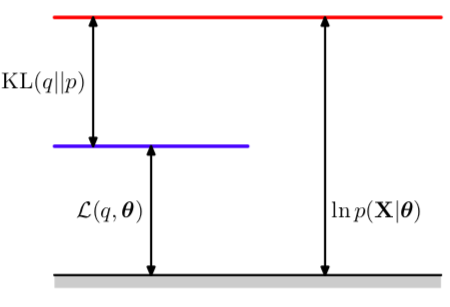
\includegraphics[width = 0.8\linewidth]{figure/figure9_11.png}
     \caption{Illustration of the decomposition given by Eqn.~\ref{decomposition}, which holds for any choice of distribution $q(\mathbf{Z}).$}
     \label{fig:9_11}
\end{figure}

The EM algorithm is a two-stage iterative optimization technique for finding maximum likelihood solutions. Suppose that the current value of the parameter vector is $\boldsymbol{\theta}^{\mathrm{old}}$.

In the E step, the lower bound $\mathcal{L}(q, \boldsymbol{\theta}^{\mathrm{old}})$ is maximized with respect to $q(\mathbf{Z})$ while holding $\boldsymbol{\theta}^{\mathrm{old}}$ fixed. The value of $\ln{p(\mathbf{X}|\boldsymbol{\theta}^{\mathrm{old}})}$ does not depend on $q(\mathbf{Z})$ and so the largest value of $\mathcal{L}(q, \boldsymbol{\theta}^{\mathrm{old}})$ will occur when the KL divergence vanishes, in other words when $q(\mathbf{Z})$ is equal to the posterior distribution $p(\mathbf{Z}|\mathbf{X}, \boldsymbol{\theta}^{\mathrm{old}})$. In this case, the lower bound will equal the log likelihood, as illustrated in Figure~\ref{fig:9_12}.

\begin{figure}[ht]
     \centering
     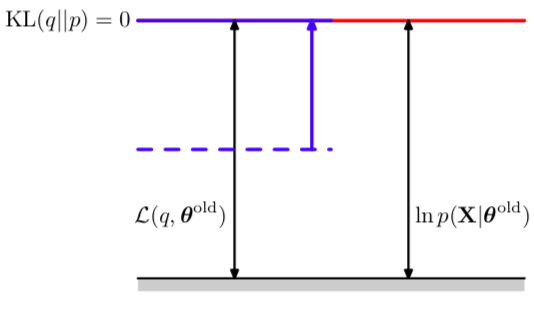
\includegraphics[width = 0.8\linewidth]{figure/figure9_12.png}
     \caption{Illustration of the E step of the EM algorithm.}
     \label{fig:9_12}
\end{figure}

In the subsequent M step, the distribution $q(\mathbf{Z})$ is held fixed and the lower bound $\mathcal{L}(q, \boldsymbol{\theta})$ is maximized with respect to $\boldsymbol{\theta}$ to give some new value $\boldsymbol{\theta}^{\mathrm{new}}$. This will cause the lower bound $\mathcal{L}$ to increase, which will necessarily cause the corresponding log likelihood function to increase. Because the distribution $q$ is determined using the old parameter values rather than the new values and is held fixed during the M step, it will not equal the new posterior distribution $p(\mathbf{Z}|\mathbf{X}, \boldsymbol{\theta}^{\mathrm{new}})$, and hence there will be a nonzero KL divergence. The increase in the log likelihood function is therefore greater than the increase in the lower bound, as shown in Figure~\ref{fig:9_13}.

\begin{figure}[ht]
     \centering
     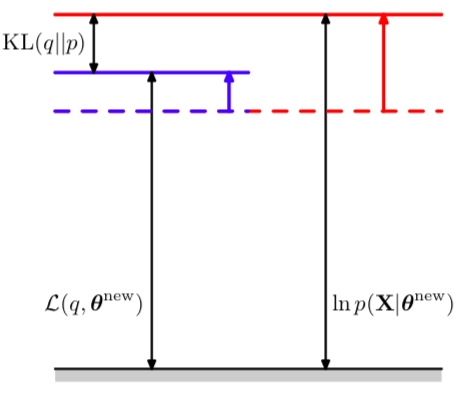
\includegraphics[width = 0.8\linewidth]{figure/figure9_13.png}
     \caption{Illustration of the M step of the EM algorithm.}
     \label{fig:9_13}
\end{figure}




%\section*{References}
\bibliography{references}

\begin{thebibliography}{9}

\bibitem{Bishop} 
Bishop, Christopher M. Pattern recognition and machine learning. springer, 2006.


\end{thebibliography}
\end{document}